%' Directed acyclic graph (DAG) with autoregressive feedback
%' 
%' @src: Last figure of the post 'Beyond Item Response Theory' 
%' @url: https://yongfu.name/2023/06/27/irt5/

\documentclass[12pt,preview,border=0]{standalone}
\usepackage[paperheight=6cm,paperwidth=15cm]{geometry}
\usepackage{graphicx}
\usepackage{amsmath}
\usepackage{kmath,kerkis}
\usepackage{tikz}
\usetikzlibrary{arrows,automata,positioning}

\begin{document} 
\begin{center}
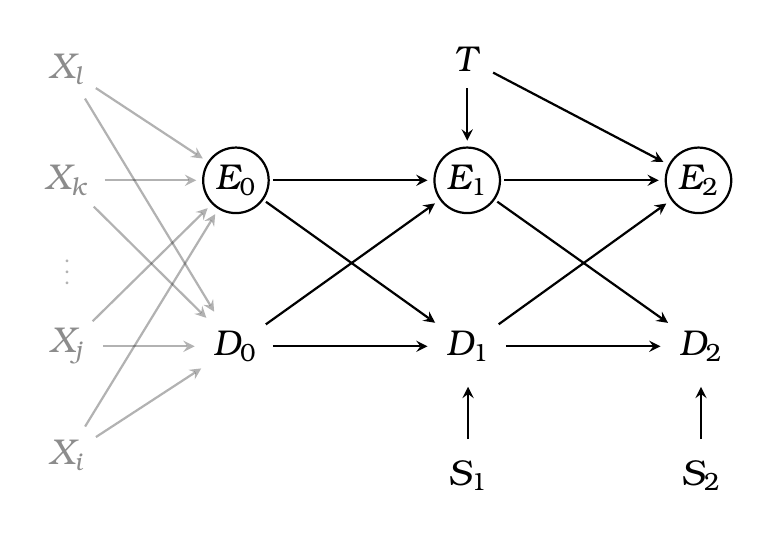
\begin{tikzpicture}[
	> = stealth, % arrow head style
	shorten > = 1pt, % don't touch arrow head to node
	auto,
	node distance = 2cm, % distance between nodes
	thick, % line style
	U/.style={circle, draw=black, inner sep=1.8pt, outer sep=1.5pt, minimum size=3mm, font=\Large},  %draw=black, fill=white
	O/.style={circle, inner sep=3.4pt, outer sep=-.75pt, minimum size=3mm, font=\Large},              %draw=white, fill=white
	]
	
	% Nodes and their relative positions
	\node[O] (X3) [opacity=.45] {$X_k$};
	\node[O] (X4) [opacity=.45, above = .5 of X3] {$X_l$};
	\node[O] (A)  [opacity=.3,  below = .2 of X3] {\small \vdots};  % phantom node
	\node[O] (X2) [opacity=.45, below = .2 of A] {$X_j$};
	\node[O] (X1) [opacity=.45, below = .5 of X2] {$X_i$};

    \node[O] (D0) [right = 1.2 of X2] {$D_0$};	
    \node[U] (E0) [right = 1.2 of X3] {$E_0$};

	\node[O] (D1) [right = of D0] {$D_1$};	
    \node[U] (E1) [right = of E0] {$E_1$};
	\node[O] (D2) [right = of D1] {$D_2$};	
    \node[U] (E2) [right = of E1] {$E_2$};

	\node[O] (T) [above = .7 of E1] {$T$};
	\node[O] (S1) [below = .7 of D1] {$S_1$};
	\node[O] (S2) [below = .7 of D2] {$S_2$};
 
	% Paths connecting nodes
	\path[->] (D0) edge (D1);
	\path[->] (D1) edge (D2);
	\path[->] (E0) edge (E1);
	\path[->] (E1) edge (E2);

	\path[->] (D0) edge (E1);
	\path[->] (D1) edge (E2);
	\path[->] (E0) edge (D1);
	\path[->] (E1) edge (D2);

	\path[->] (S1) edge (D1);
	\path[->] (S2) edge (D2);

	\path[->] (T) edge (E1);
	\path[->] (T) edge (E2);

	\path[->] (X1) edge[opacity=0.3] (E0);
	\path[->] (X1) edge[opacity=0.3] (D0);
	\path[->] (X2) edge[opacity=0.3] (E0);
	\path[->] (X2) edge[opacity=0.3] (D0);
	\path[->] (X3) edge[opacity=0.3] (E0);
	\path[->] (X3) edge[opacity=0.3] (D0);
	\path[->] (X4) edge[opacity=0.3] (E0);
	\path[->] (X4) edge[opacity=0.3] (D0);

\end{tikzpicture}
\end{center}

\end{document}
